\documentclass[12pt]{article}
\usepackage{amsmath}
\usepackage{graphicx}
\usepackage{hyperref}
\usepackage[utf8]{inputenc}
\usepackage{geometry}
\usepackage{mathtools}
\usepackage{empheq}
\usepackage{listings}
\usepackage{xcolor}
\usepackage{minted}
\usepackage{siunitx}
\definecolor{LightGray}{gray}{0.9}

\graphicspath{ {./assets/} }
\geometry{margin=0.75in}

\title{CHEN 425 HW2}
\author{Mark Levchenko}
\date{January 2023}

\begin{document}

\begin{enumerate}
% Problem 1 %%%%%%%%%%%%%%%%%%%%%%%%%%%%%%%%%%%%%%%%%%%%%%%%%%%%%%%%%%%%
    \item Problem 2.13
    \begin{align*}
        V_0 &= \$ 50 \text{ MM} \\
        V_S &= \$ 50 \text{ MM} \cdot \% 10 = \$ 5 \text{ MM}  \\
        d &= \frac{\$ 50 \text{ MM} - \$ 5 \text{ MM}}{10} \\
        \Aboxed{d &= \$ 4.5 \text{ MM} / \mathrm{yr}}
    \end{align*}

% Problem 2 %%%%%%%%%%%%%%%%%%%%%%%%%%%%%%%%%%%%%%%%%%%%%%%%%%%%%%%%%%%%
\newpage
    \item Problem 2.14
    \begin{enumerate}
    \item
    \begin{align*}
        \mathrm{FCI} &= \$ 28 \text{ MM} \\
        \mathrm{salvage} &= \$ 3 \text{ MM} \\
        N &= 10 \\
        \alpha &= \frac{2}{10} = 0.2 \\
    \end{align*}

    DDB method with linear adjustment in the final year:

    \begin{tabular}{|c|c|c|}
        \hline
        Year & Depreciation charge (\$ MM) & Book Value (\$ MM) \\
        \hline
        0 & 0 & 28 \\
        1 &	5.6 & 22.4 \\
        2 &	4.48 & 17.92 \\
        3 &	3.58 & 14.33 \\
        4 &	2.86 & 11.46 \\
        5 &	2.29 & 9.17 \\
        6 &	1.83 & 7.34 \\
        7 &	1.46 & 5.87 \\
        8 &	1.17 & 4.69 \\
        9 &	0.93 & 3.75 \\
        10 & 0.75 & 3 \\
        \hline
    \end{tabular}
    


    \item Straight line depreciation:
    
    \begin{tabular}{|c|c|c|}
        \hline
        Year & Depreciation charge (\$ MM) & Book Value (\$ MM) \\
        \hline
        0 & 0 & 28 \\
        1 & 2.5 & 25.5 \\
        2 & 2.5 & 23 \\
        3 & 2.5 & 20.5 \\
        4 & 2.5 & 18 \\ 
        5 & 2.5 & 15.5 \\
        6 & 2.5 & 13 \\
        7 & 2.5 & 10.5 \\
        8 & 2.5 & 8 \\
        9 & 2.5 & 5.5 \\
        10 & 2.5 & 3 \\
        \hline
    \end{tabular}

    Comparison plot:

    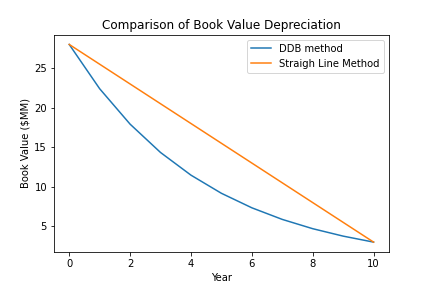
\includegraphics{CHEN425_HW2_2.14_fig.png}

    \end{enumerate}
    

% Problem 3 %%%%%%%%%%%%%%%%%%%%%%%%%%%%%%%%%%%%%%%%%%%%%%%%%%%%%%%%%%%%
\newpage
    \item Problem 2.15

    Five year MACRS depreciation:

    \begin{tabular}{|c|c|c|}
        \hline
        Year & Book Value (\$ MM) & Depreciation charge (\$ MM) \\
        \hline
        0 & 100.00 & 0.00 \\
        1 & 80.00 & 20.00 \\
        2 & 48.00 & 32.00 \\ 
        3 & 28.80 & 19.20 \\
        4 & 17.28 & 11.52 \\
        5 & 5.76 & 11.52 \\ 
        6 & 0.00 & 5.76 \\
        \hline
    \end{tabular}

    Ten year MACRS depreciation:

    \begin{tabular}{|c|c|c|}
        \hline
        Year & Book Value (\$ MM) & Depreciation charge (\$ MM) \\
        \hline
        0 & 100.00 & 0.00 \\
        1 & 90.00 & 10.00 \\
        2 & 72.00 & 18.00 \\
        3 & 57.60 & 14.40 \\
        4 & 46.08 & 11.52 \\
        5 & 36.86 & 9.21 \\
        6 & 29.49 & 7.37 \\
        7 & 22.93 & 6.55 \\
        8 & 16.38 & 6.55 \\
        9 & 9.83 & 6.55	\\
        10 & 3.27 & 6.55 \\
        11 & 0.00 & 3.27 \\
        \hline
    \end{tabular}

    When depreciated over five years, linear depreciation begins in the fourth year. When depreciated over ten years, linear depreciation begins in the seventh year. The unit is depreciated to zero because the MACRS method does not care about salvage value. Most of the book value is depreciated in the first few years of depreciation.

    \newpage
    Comparison plot:

    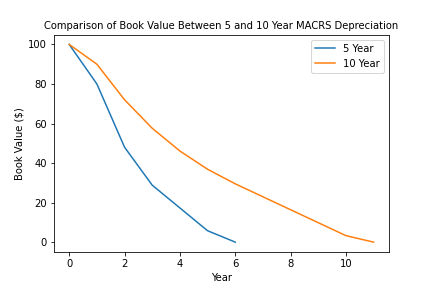
\includegraphics{CHEN425_HW2_2.15_fig.png}


\end{enumerate}

\end{document}
